% THIS IS SIGPROC-SP.TEX - VERSION 3.1
% WORKS WITH V3.2SP OF ACM_PROC_ARTICLE-SP.CLS
% APRIL 2009
%
% Questions regarding SIGS should be sent to
% Adrienne Griscti ---> griscti@acm.org
%
% Questions/suggestions regarding the guidelines, .tex and .cls files, etc. to
% Gerald Murray ---> murray@hq.acm.org
%
% For tracking purposes - this is V3.1SP - APRIL 2009
%
% Copied from https://github.com/heathermiller/papers-documents/tree/master/rem2013

\documentclass{support/acm_proc_article-sp}
\usepackage{listings}
\usepackage{url}
\usepackage{support/bcprules}
\usepackage{support/prooftree}
\usepackage{support/math}
\usepackage{multicol}
\usepackage{caption}
\usepackage{subcaption}
\usepackage[normalem]{ulem}
\usepackage{color}
\usepackage{graphicx}
\usepackage{hyperref}

\renewcommand{\thesubsection}{\thesection.\alph{subsection}}

\definecolor{blue}{rgb}{0,0,0.5}
\definecolor{red}{rgb}{0.6,0,0}
\definecolor{green}{rgb}{0,0.5,0}
\definecolor{grey}{rgb}{0.2,0.2,0.2}

\lstdefinelanguage{Python}{
keywords={typeof, null, catch, switch, in, int, str, float, self, from, import},
keywordstyle=\color{blue}\bfseries,
ndkeywords={boolean, throw, import},
ndkeywords={return, class, if ,elif, endif, while, do, else, True, False , catch, def},
ndkeywordstyle=\color{blue}\bfseries,
identifierstyle=\color{grey},
sensitive=false,
comment=[l]{\#},
morecomment=[s]{/*}{*/},
commentstyle=\color{green}\ttfamily,
stringstyle=\color{green}\ttfamily,
}

\lstset{language=Python}

\clubpenalty = 10000
\widowpenalty = 10000
\displaywidowpenalty = 10000

% Remove copyright space
\makeatletter
\def\@copyrightspace{\relax}
\makeatother

% comments and notes
\newcommand{\comment}[1]{}
\newcommand{\note}[1]{{\bf $\clubsuit$ #1 $\spadesuit$}}
\newcommand{\ifreport}[1]{#1}
%\newcommand{\ifreport}[1]{}

\newcommand{\todo}{{\bf \colorbox{red}{\color{white}TODO:}}}
\newcommand{\ie}{{\em i.e.,~}}
\newcommand{\eg}{{\em e.g.,~}}
\newcommand{\term}[1]{\mbox{\texttt{#1}}}
\newcommand{\itl}[1]{\mbox{\textit{#1}}}

% commas and semicolons
\newcommand{\comma}{,\,}
\newcommand{\commadots}{\comma \ldots \comma}
\newcommand{\semi}{;\mbox{;};}
\newcommand{\semidots}{\semi \ldots \semi}

% spacing
\newcommand{\gap}{\quad\quad}
\newcommand{\biggap}{\quad\quad\quad}
\newcommand{\nextline}{\\ \\}
\newcommand{\htabwidth}{0.5cm}
\newcommand{\tabwidth}{1cm}
\newcommand{\htab}{\hspace{\htabwidth}}
\newcommand{\tab}{\hspace{\tabwidth}}
\newcommand{\linesep}{\ \hrulefill \ \smallskip}

\newcommand{\sectionline}{%
\nointerlineskip \vspace{\baselineskip}%
\hspace{\fill}\rule{0.5\linewidth}{.7pt}\hspace{\fill}%
\par\nointerlineskip \vspace{\baselineskip}
}

% figures
\newcommand{\figurebox}[1]
{\fbox{\begin{minipage}{\textwidth}
           #1 \medskip
\end{minipage}}}
\newcommand{\twofig}[3]
{\begin{figure*}[t]
     #3\ \hrulefill\
        \caption{\label{#1}#2}
\end{figure*}}
\newcommand{\boxfig}[3]
{\begin{figure*}
     \figurebox{#3\caption{\label{#1}#2}}
\end{figure*}}
\newcommand{\figref}[1]
{Figure~\ref{#1}}

% arrays
\newcommand{\ba}{\begin{array}}
\newcommand{\ea}{\end{array}}
\newcommand{\bda}{\[\ba}
\newcommand{\eda}{\ea\]}
\newcommand{\ei}{\end{array}}
\newcommand{\bcases}{\left\{\begin{array}{ll}}
\newcommand{\ecases}{\end{array}\right.}

\pagenumbering{arabic}
\begin{document}

    \title{Data Mining and Matrices (FSS18) \\ Assignment 2: Matrix Completion}

    \numberofauthors{1}
    \author{
    \alignauthor
    Steffen Schmitz\\
    \affaddr{University of Mannheim}\\
    \affaddr{stefschm@mail.uni-mannheim.de}
    }

    \maketitle

    %%%%%%%%%%%%%%%%%%%%%%%%%%%%%%%%%%%%%%%%%%%%%%%%%%%%
    %%
    %% 1) Computing the Loss Function
    %%
    %%%%%%%%%%%%%%%%%%%%%%%%%%%%%%%%%%%%%%%%%%%%%%%%%%%%

    \section{Computing the Loss Function}
    \label{sec:loss-function}

    In this assignment, we will make use of the following loss function:
    \begin{equation}
        L(\mathbf{L}, \mathbf{R}) = \sum_{(i,j)\in \Omega} (d_{ij} - [\mathbf{LR}]_{ij})^2
            + \frac{\lambda}{2}(\Vert \mathbf{L} \Vert_F^2 + \Vert \mathbf{R} \Vert_F^2)
        \label{eq:loss-matrix}
    \end{equation}
    \begin{equation}
        = \sum_{(i,j)\in \Omega} \left[ (d_{ij} - \mathbf{l}_i^T \mathbf{r}_j)^2
            + \frac{\lambda \Vert \mathbf{l}_i \Vert_2^2}{2N_i}
            + \frac{\lambda \Vert \mathbf{r}_j \Vert_2^2}{2N_j} \right]
        \label{eq:loss-vector}
    \end{equation}
    \begin{equation}
        = \sum_{(i,j)\in \Omega} \left[ \left(d_{ij} - \sum_{k=1}^r l_{ik}r_{kj} \right)^2
        + \frac{\lambda\sum_{k=1}^r l_{ik}^2}{2N_i}
        + \frac{\lambda\sum_{k=1}^r r_{kj}^2}{2N_j} \right]
        \label{eq:loss-scalar}
    \end{equation}
    This loss function computes the squared error in reconstructing the revealed
    entries in $\mathbf{D}$, plus an L2 regularization term.

    %%%%%%%%%%%%%%%%%%%%%%%%%%%%%%%%%%%%%%%%%%%%%%%%%%%%
    %%
    %% 1.a) Prove the Equality
    %%
    %%%%%%%%%%%%%%%%%%%%%%%%%%%%%%%%%%%%%%%%%%%%%%%%%%%%

    \subsection{Prove the Equality}

    \textbf{Task.} Prove that the above equalities hold.

    In order to prove the equalities of Equation \ref{eq:loss-matrix}, \ref{eq:loss-vector} and
    \ref{eq:loss-scalar} hold, we split them into two parts.
    First, we show that the local loss, $\sum_{(i,j)\in\Omega}(d_{ij} - [\mathbf{LR}]_{ij})^2$,
    is equivalent to the first part of the second and third equation and afterwards we will show
    that the reformulations of the L2 regularization, $\frac{\lambda}{2}(\Vert \mathbf{L} \Vert_F^2 +
    \Vert \mathbf{R} \Vert_F^2)$ are equivalent.

    For the local loss we need to show that
    \begin{equation*}
        (d_{ij} - [\mathbf{LR}]_{ij})^2 =
        (d_{ij} - \mathbf{l}_i^T \mathbf{r}_j)^2 =
        \left(d_{ij} - \sum_{k=1}^r l_{ik}r_{kj} \right)^2
    \end{equation*}
    for any $(i,j)\in\Omega$.
    If this equality holds for an arbitrary pair of revealed entries it holds for the complete
    sum.
    By taking the square root, subtracting $d_{ij}$ and multiplying it by $-1$ we get the following statement
    \begin{equation*}
        [\mathbf{LR}]_{ij} =
        \mathbf{l}_i^T \mathbf{r}_j =
        \sum_{k=1}^r l_{ik}r_{kj}
    \end{equation*}
    which is exactly the result of a multiplication for entry $(i,j)$ as defined in the lecture.

    Second, the equalities for the L2 regularization must hold.
    They are shown in Equation \ref{eq:l2-reg-1} and \ref{eq:l2-reg-2}.
    \begin{equation}
        \frac{\lambda}{2}(\Vert \mathbf{L} \Vert_F^2 + \Vert \mathbf{R} \Vert_F^2)
        = \sum_{(i,j)\in \Omega} \left( \frac{\lambda \Vert \mathbf{l}_i \Vert_2^2}{2N_i}
            + \frac{\lambda \Vert \mathbf{r}_j \Vert_2^2}{2N_j} \right)
        \label{eq:l2-reg-1}
    \end{equation}
    \begin{equation}
        \frac{\lambda}{2}(\Vert \mathbf{L} \Vert_F^2 + \Vert \mathbf{R} \Vert_F^2)
        = \sum_{(i,j)\in \Omega} \left( \frac{\lambda\sum_{k=1}^r l_{ik}^2}{2N_i}
        + \frac{\lambda\sum_{k=1}^r r_{kj}^2}{2N_j} \right)
        \label{eq:l2-reg-2}
    \end{equation}
    $\frac{\lambda}{2}$ is a constant in all terms and, therefore, we can cancel it out.
    Splitting the equations into $\mathbf{L}$ and $\mathbf{R}$ related terms, we obtain
    \begin{equation*}
        \Vert \mathbf{L} \Vert_F^2
        = \frac{1}{N_i}\sum_{(i,j)\in \Omega} \Vert \mathbf{l}_i \Vert_2^2
        = \frac{1}{N_i}\sum_{(i,j)\in \Omega} \sum_{k=1}^r l_{ik}^2
    \end{equation*}
    and
    \begin{equation*}
        \Vert \mathbf{R} \Vert_F^2
        = \frac{1}{N_j}\sum_{(i,j)\in \Omega} \Vert \mathbf{r}_j \Vert_2^2
        = \frac{1}{N_j}\sum_{(i,j)\in \Omega} \sum_{k=1}^r r_{kj}^2
    \end{equation*}

    The Frobenius norm, defined as $\Vert A\Vert_F = \sqrt{\sum_{i = 1}^m \sum_{j=1}^n a_{ij}^2}$, is the same as
    the two outer terms in both equations, taking the square into account.
    $\frac{1}{N_{i/j}}$ serves as a normalization constant that is only required, because we are looking at a subset of
    the rows and columns of $\mathbf{L}$ and $\mathbf{R}$, respectively.

    Now the only equality left to show is that
    \begin{equation*}
        \Vert \mathbf{L} \Vert_F^2
        = \frac{1}{N_i}\sum_{(i,j)\in \Omega} \Vert \mathbf{l}_i \Vert_2^2
    \end{equation*}
    and
    \begin{equation*}
        \Vert \mathbf{R} \Vert_F^2
        = \frac{1}{N_j}\sum_{(i,j)\in \Omega} \Vert \mathbf{r}_j \Vert_2^2
    \end{equation*}
    As in the exercise for matrix completion, we can use the fact that $\Vert A\Vert_F^2 = \sum_i\Vert a_i\Vert_2^2$.
    Treating $\frac{1}{N_{i/j}}$ as a normalization constant again we can see that this equality, too, holds.

    We, therefore, have shown that Equation \ref{eq:loss-matrix}, \ref{eq:loss-vector} and
    \ref{eq:loss-scalar} are equivalent.

    %%%%%%%%%%%%%%%%%%%%%%%%%%%%%%%%%%%%%%%%%%%%%%%%%%%%
    %%
    %% 2) Computing the Local Gradients
    %%
    %%%%%%%%%%%%%%%%%%%%%%%%%%%%%%%%%%%%%%%%%%%%%%%%%%%%

    \section{Computing the Local Gradients}

    %%%%%%%%%%%%%%%%%%%%%%%%%%%%%%%%%%%%%%%%%%%%%%%%%%%%
    %%
    %% 2.a) Gradient per Entry
    %%
    %%%%%%%%%%%%%%%%%%%%%%%%%%%%%%%%%%%%%%%%%%%%%%%%%%%%

    \subsection{Gradient per Entry}
    \label{subsec:gradient-entry}

    \textbf{Task.} Set
    \begin{equation*}
        \begin{aligned}
            L_{ij}(\mathbf{l}_i,\mathbf{r}_j) & = (d_{ij} - \mathbf{l}_i^T \mathbf{r}_j)^2
                                                + \frac{\lambda \Vert \mathbf{l}_i \Vert_2^2}{2N_i}
                                                + \frac{\lambda \Vert \mathbf{r}_j \Vert_2^2}{2N_j} \\
                                              & = \left(d_{ij} - \sum_{k=1}^r l_{ik}r_{kj} \right)^2
                                                + \frac{\lambda\sum_{k=1}^r l_{ik}^2}{2N_i}
                                                + \frac{\lambda\sum_{k=1}^r r_{kj}^2}{2N_j}
        \end{aligned}
    \end{equation*}
    as in (\ref{eq:loss-vector}) and (\ref{eq:loss-scalar}).
    Compute the gradients w.r.t.\@ to each entry in the factor matrices, i.e.\@, compute
    \begin{equation*}
        \begin{aligned}
            \nabla_{l_{ik}}L_{ij}(\mathbf{l}_i,\mathbf{r}_j),\\
            \nabla_{r_{kj}}L_{ij}(\mathbf{l}_i,\mathbf{r}_j).
        \end{aligned}
    \end{equation*}

    First, we compute the gradient with regards to $l_{ik}$ which we can write as
    \begin{equation*}
        \begin{aligned}
            \nabla_{l_{ik}}L_{ij}(\mathbf{l}_i,\mathbf{r}_j)
                & = \nabla_{l_{ik}} \left(d_{ij} - \sum_{k=1}^r l_{ik}r_{kj} \right)^2 \\
                & + \nabla_{l_{ik}} \frac{\lambda\sum_{k=1}^r l_{ik}^2}{2N_i} \\
                & + \nabla_{l_{ik}} \frac{\lambda\sum_{k=1}^r r_{kj}^2}{2N_j}
        \end{aligned}
    \end{equation*}
    using the sum-rule.
    The last term does not depend on $l_{ik}$, can, therefore, be treated as a constant, and becomes $0$ in the
    derivative.
    In the second summand we can factor out $\frac{\lambda}{2N_i}$ and are left with $\nabla_{l_{ik}}\sum_{k=1}^r l_{ik}^2$
    which is equal to $2\cdot\sum_{k=1}^r l_{ik}$.
    This leaves us with
    \begin{equation*}
        \nabla_{l_{ik}}L_{ij}(\mathbf{l}_i,\mathbf{r}_j) = \nabla_{l_{ik}} \left(d_{ij} - \sum_{k=1}^r l_{ik}r_{kj} \right)^2
                                                         + \frac{\lambda}{N_i}\sum_{k=1}^r l_{ik}
    \end{equation*}
    Finally, we apply the chain rule and get
    \begin{equation*}
        \nabla_{l_{ik}}L_{ij}(\mathbf{l}_i,\mathbf{r}_j) =
            -2\cdot(d_{ij} - \sum_{k=1}^r l_{ik}r_{kj}) \cdot (\sum_{k=1}^r r_{kj})
            + \frac{\lambda}{N_i}\sum_{k=1}^r l_{ik}
    \end{equation*}
    Similarly we get as the result for $\nabla_{r_{kj}}L_{ij}(\mathbf{l}_i,\mathbf{r}_j)$
    \begin{equation*}
        \nabla_{r_{kj}}L_{ij}(\mathbf{l}_i,\mathbf{r}_j) =
        -2\cdot(\sum_{k=1}^r l_{ik})\cdot(d_{ij} - \sum_{k=1}^r l_{ik}r_{kj})
        + \frac{\lambda}{N_j}\sum_{k=1}^r r_{kj}
    \end{equation*}

    %%%%%%%%%%%%%%%%%%%%%%%%%%%%%%%%%%%%%%%%%%%%%%%%%%%%
    %%
    %% 2.b) Gradient per Row/Column
    %%
    %%%%%%%%%%%%%%%%%%%%%%%%%%%%%%%%%%%%%%%%%%%%%%%%%%%%

    \subsection{Gradient per Row/Column}

    \textbf{Task.} Compute the gradients w.r.t.\@ to each row/column in the factor matrices,
    i.e.\@, compute
    \begin{equation*}
        \begin{aligned}
            \nabla_{\mathbf{l}_i^T}L_{ij}(\mathbf{l}_i,\mathbf{r}_j),\\
            \nabla_{\mathbf{r}_j^T}L_{ij}(\mathbf{l}_i,\mathbf{r}_j).
        \end{aligned}
    \end{equation*}

    For this subtask we can reuse the results from Section \ref{subsec:gradient-entry} and replace the sums over
    $k$ values with a vectorized computation.
    This results in the following equation for $\nabla_{\mathbf{l}_i^T}L_{ij}(\mathbf{l}_i,\mathbf{r}_j)$
    \begin{equation*}
        \nabla_{\mathbf{l}_i^T}L_{ij}(\mathbf{l}_i,\mathbf{r}_j) =
        -2\cdot(d_{ij} - \mathbf{l}_i^T \mathbf{r}_j) \cdot \mathbf{r}_j^T
        + \frac{\lambda}{N_i} \mathbf{l}_i^T
    \end{equation*}
    and for $\nabla_{\mathbf{r}_j^T}L_{ij}(\mathbf{l}_i,\mathbf{r}_j)$
    \begin{equation*}
        \nabla_{\mathbf{r}_j^T}L_{ij}(\mathbf{l}_i,\mathbf{r}_j) =
        -2\cdot\mathbf{l}_i^T\cdot(d_{ij} - \mathbf{l}_i^T \mathbf{r}_j)
        + \frac{\lambda}{N_j} \mathbf{r}_j^T
    \end{equation*}

    %%%%%%%%%%%%%%%%%%%%%%%%%%%%%%%%%%%%%%%%%%%%%%%%%%%%
    %%
    %% 3) Implementing Gradient Descent
    %%
    %%%%%%%%%%%%%%%%%%%%%%%%%%%%%%%%%%%%%%%%%%%%%%%%%%%%

    \section{Implementing Gradient Descent}

    \textbf{Task.} Complete the function \lstinline{gdepoch}.
    Once this function is implemented, you are ready to factorize the provided image.
    The default choice of parameters in the R script is $r = 10$ and $\lambda = 2$.
    Run gradient descent by executing the commands provided in the R script.
    Visualize the result after 5, 15, and 50 epochs and discuss.

    The goal of our implementation is to compute an estimation of the full matrix, based on the revealed entries.
    In contrast to the Singular Value Decomposition, we only take revealed entries into account and ignore
    missing values completely.

    We try to minimize the loss function from Section \ref{sec:loss-function} by the application of Gradient Descent.
    Therefore, we compute the gradient at a random point and walk downhill towards a minimum.
    After each step (epoch) we are closer to the minimum and our approximation of the matrix should become better.
    The first approximation after 5 epochs is shown in Figure \ref{fig:gradient-5}.
    \begin{figure}[htbp]
        \centering
        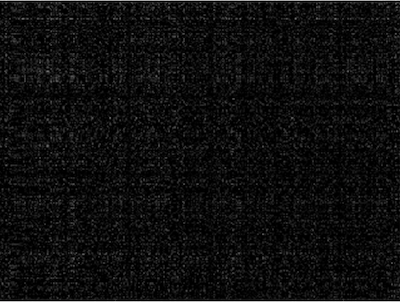
\includegraphics[width=8cm]{images/gradient-5.png}
        \caption{Matrix factorization after 5 epochs}
        \label{fig:gradient-5}
    \end{figure}
    We can only see a few grey dots on a black background without the possibility to identify any shapes in the picture.
    At this point we are still far away from the best factorization and observe a high error between the
    original matrix $\mathbf{D}$ and the rank $r$ factorization $\mathbf{LR}$.

    Figure \ref{fig:gradient-15} visualizes the factorization after 15 epochs of gradient descent.
    \begin{figure}[htbp]
        \centering
        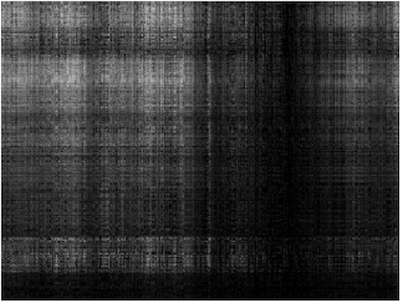
\includegraphics[width=8cm]{images/gradient-15.png}
        \caption{Matrix factorization after 15 epochs}
        \label{fig:gradient-15}
    \end{figure}
    It includes shapes that are clearly distinguishable and, with having in mind, that the original image shows three persons
    with sunglasses and a label at the bottom we can make out the basic shapes of all of these.
    The factorization after 15 epochs is much better than after 5.
    It reconstructs the basic structure of the image without showing any details.

    Finally, we look at the factorization after running 50 epochs of gradient descent.
    \begin{figure}[htbp]
        \centering
        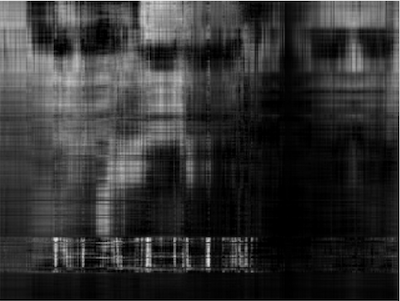
\includegraphics[width=8cm]{images/gradient-50.png}
        \caption{Matrix factorization after 50 epochs}
        \label{fig:gradient-50}
    \end{figure}
    The image in Figure \ref{fig:gradient-50} clearly resembles the original image with unrevealed entries.
    We can clearly identify three persons and the "Matrix" text in the bottom left.
    The difference between the original image with unrevealed entries and the factorization $\mathbf{LR}$ seems
    very small.

    Yet, there still is a lot of noise in the image.
    Running gradient descent for image completion is a suboptimal method, because it does not take the relation between
    neighbouring pixels into account.
    Another factor is that we only compute a rank $r$ approximation instead of a perfect factorization.

    Looking at the computed error in each epoch we can see that it sharply falls in the beginning, but the improvement
    continues to decline with each epoch.
    Approaching the minimum, it becomes harder to optimize the image even further without increasing the loss elsewhere.

    All in all, we draw the conclusion that the gradient descent approach produces a good factorization for the sparse
    matrix $\mathbf{D}$.

    %%%%%%%%%%%%%%%%%%%%%%%%%%%%%%%%%%%%%%%%%%%%%%%%%%%%
    %%
    %% 4) Implementing Stochastic Gradient Descent
    %%
    %%%%%%%%%%%%%%%%%%%%%%%%%%%%%%%%%%%%%%%%%%%%%%%%%%%%

    \section{Implementing Stochastic Gradient Descent}

    \textbf{Task.} Factorize the matrix again, this time using stochastic gradient descent (as before, set
    $r = 10$ and $\lambda = 2$).
    Compare the result with the result obtained by gradient descent and discuss.

    The resulting factorization $\mathbf{LR}$ for matrix $\mathbf{D}$ is shown in Figure \ref{fig:sgradient}.
    \begin{figure}[htbp]
        \centering
        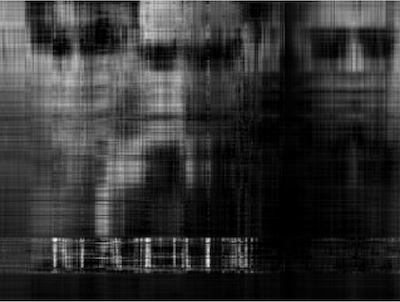
\includegraphics[width=8cm]{images/sgradient.png}
        \caption{Matrix factorization with Stochastic Gradient Descent}
        \label{fig:sgradient}
    \end{figure}
    As in Figure \ref{fig:gradient-50}, we see three persons with sunglasses and the "Matrix" label in the bottom
    left of the image.
    Both images look very similar, which means that both methods found the same minimum of the error function.

    From the error per epoch in the notebook we also derive that they start with the same error and finish of at a similar
    error that is around 415.
    The errors of corresponding epochs are closely together.

    This result is expected, because the stochastic gradient descent should approximate converge to the same
    optimum as the gradient descent, especially when the Loss function is convex.

    %%%%%%%%%%%%%%%%%%%%%%%%%%%%%%%%%%%%%%%%%%%%%%%%%%%%
    %%
    %% 5) Impact of Parameter Choices
    %%
    %%%%%%%%%%%%%%%%%%%%%%%%%%%%%%%%%%%%%%%%%%%%%%%%%%%%

    \section{Impact of Parameter Choices}

    \textbf{Task.} Factorize the input matrix with the following choice of parameters (using either gradient descent
    or stochastic gradient descent):
    \begin{itemize}
        \item $r = 10$, $\lambda = 2$ (mildly regularized),
        \item $r = 10$, $\lambda = 0$ (unregularized),
        \item $r = 10$, $\lambda = 20$ (heavily regularized),
        \item $r = 1$, $\lambda = 0$ (lower rank),
        \item $r = 20$, $\lambda = 2$ (higher rank).
    \end{itemize}
    Compare the resulting completed matrices visually.
    What is the effect of the various parameters?
    Discuss.

    For this section we compute all results with stochastic gradient descent.

    The first parameter combination we look at are the parameters that we have used across all previous sections.
    \begin{figure}[htbp]
        \centering
        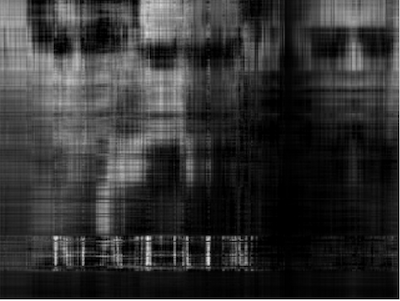
\includegraphics[width=8cm]{images/sgd_r10_l2.png}
        \caption{Mildly regularized matrix factorization}
        \label{fig:sgd_r10_l2}
    \end{figure}
    It uses rank $r = 10$ and $\lambda = 2$, which means that the factorization is mildly regularized.
    This again means that we apply a small penalty if the magnitude of the matrices $\mathbf{L}$ and $\mathbf{R}$
    becomes large.
    The result in Figure \ref{fig:sgd_r10_l2} demonstrates, as expected, a similar image to the ones in the previous chapters.

    In Figure \ref{fig:sgd_r10_l0} we remove the regularization and only minimize the error between the original
    matrix and our factorization.
    \begin{figure}[htbp]
        \centering
        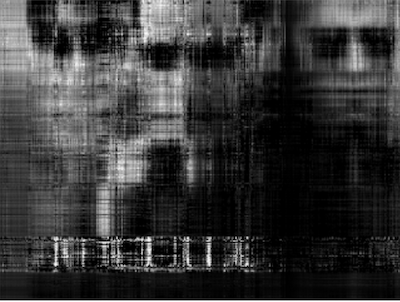
\includegraphics[width=8cm]{images/sgd_r10_l0.png}
        \caption{Unregularized matrix factorization}
        \label{fig:sgd_r10_l0}
    \end{figure}
    In the picture we observe brighter spots than before and a greater variation of colors.
    Especially the more prominent features of the left two faces, like the noses and the cheekbones have a color closer
    to white than in the mildly regularized image.

    As the regularization imposes a penalty on large values this is expected.
    The absence of this regularisation allows the factorization to minimize the error even further by increasing
    the values in some spots.
    This is a common consequence of overfitting the dataset and one of the reasons why regularization is
    applied \cite[cf. p.227]{Murphy:2012}.

    The next parameter combination applies a heavy penalty for large matrix norms of $\mathbf{L}$ and $\mathbf{R}$.
    The resulting image is displayed in Figure \ref{fig:sgd_r10_l20}.
    \begin{figure}[htbp]
        \centering
        
\includegraphics[width=8cm]{images/sgd_r10_l20.png}
        \caption{Heavily regularized matrix factorization}
        \label{fig:sgd_r10_l20}
    \end{figure}
    We are able to single out the basic outlines of the three characters in the image, but, overall, very little gets revealed.
    Instead of overfitting the image like in Figure \ref{fig:sgd_r10_l0}, we underfit it, which means that the penalty
    on the matrices is so high that they are not flexible enough to capture the essence of the original
    matrix $\mathbf{D}$.

    The last two parameter combinations focus on the rank of the matrix instead of the regularization parameter $\lambda$.
    A low rank corresponds to a rather simple matrix, because all rows and columns have to be linear combinations of another,
    while a high rank allows the matrix to be more complex.

    The matrix factorization for rank 1 is visualized in Figure \ref{fig:sgd_r1_l0}.
    The shapes look similar to the gradient descent result after 15 epochs from Figure \ref{fig:gradient-15}.
    \begin{figure}[htbp]
        \centering
        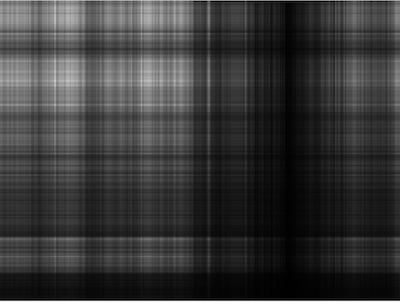
\includegraphics[width=8cm]{images/sgd_r1_l0.png}
        \caption{Lower rank matrix factorization}
        \label{fig:sgd_r1_l0}
    \end{figure}
    We can also observe that the image consists exclusively of straight lines without any clearly distinguishable pixels.
    This is the case, because every row and column is a linear combination and, thus, it is not possible to create any shapes,
    except through intersections of weighted lines.

    On the opposite side, we have the high rank factorization in Figure \ref{fig:sgd_r20_l2}, which captures many details.
    \begin{figure}[htbp]
        \centering
        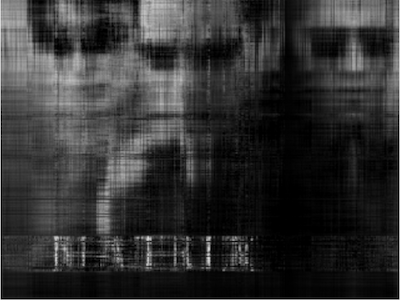
\includegraphics[width=8cm]{images/sgd_r20_l2.png}
        \caption{Higher rank matrix factorization}
        \label{fig:sgd_r20_l2}
    \end{figure}
    The image looks similar to the mildly regularized image in Figure \ref{fig:sgd_r10_l2}, but makes some minor
    improvements around the "Matrix" label on the bottom left.
    With the additional complexity that is allowed through the higher rank it improves on some structures, but is still
    similar to the rank 10 image.

    All in all, the choice of the parameters $r = 10$ and $\lambda = 2$ seems the most reasonable, as the resulting
    image contains all important structures and, at the same time, is not very complex.

    %%%%%%%%%%%%%%%%%%%%%%%%%%%%%%%%%%%%%%%%%%%%%%%%%%%%
    %%
    %% BIBLIOGRAPHY
    %%
    %%%%%%%%%%%%%%%%%%%%%%%%%%%%%%%%%%%%%%%%%%%%%%%%%%%%

    \bibliographystyle{abbrv}
    \bibliography{support/bib}

\end{document}
